% Chapter 5
\label{Capítulo5}
\chapter{Resultados}
\begin{center}
    \textit{``Newton's third law. You've got to leave something behind''}
     
     Cooper
\end{center}

\section{Lei de \textit{Ohm}}
\label{sec:resultados_lei_de_ohm}
\textbf{Falta o complemento com imagens do gráfico/resultado final e a imagem da placa já feita, opinião PROF}

Na forma da Equação \ref{eq:leideohm}, a Lei de \textit{Ohm} estabelece que a resistência eléctrica ($R$) de um condutor é determinada pelo quociente entre a tensão elétrica ($U$) aplicada aos seus terminais e a corrente eléctrica ($I$) que o atravessa.  

\begin{equation} \label{eq:leideohm}
	R=\dfrac{U}{I}
\end{equation}

Isto significa que a Equação \ref{eq:leideohm} define uma relação linear entre a tensão e a corrente para uma determinada resistência de valor fixo, o que implica que o gráfico obtido, representado na Figura \ref{fig:graphohm}, é uma linha recta que passa pela origem. O declive dessa recta representa o valor da resistência elétrica ($R$).

\begin{figure}[hbtp]
	\centering
	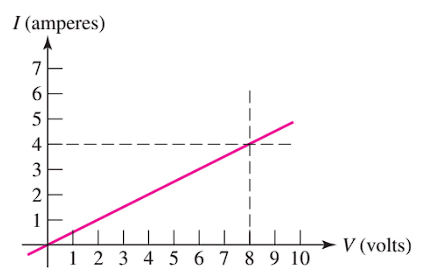
\includegraphics[width=0.3\textwidth]{figures/grafico_Ohm.png}
	\caption{Gráfico da Lei de \textit{Ohm}}
	\label{fig:graphohm}
\end{figure}

Da forma como foi implementado, há duas possibilidades de realizar este estudo, exemplificado nas Figuras \ref{fig:Opção_1} e \ref{fig:Opção_2}. No entanto, no contexto desta dissertação foi  implementado o caso descrito na Figura \ref{fig:Opção_1}\footnote{Como trabalho futuro, o menu poderia ser desenvolvido para o utilizador, aluno ou professor escolher a opção pretendida.}. 

\begin{figure}[hbtp]
	\centering%
		\centering
		\subfloat[\centering Opção 1\label{fig:Opção_1}]{{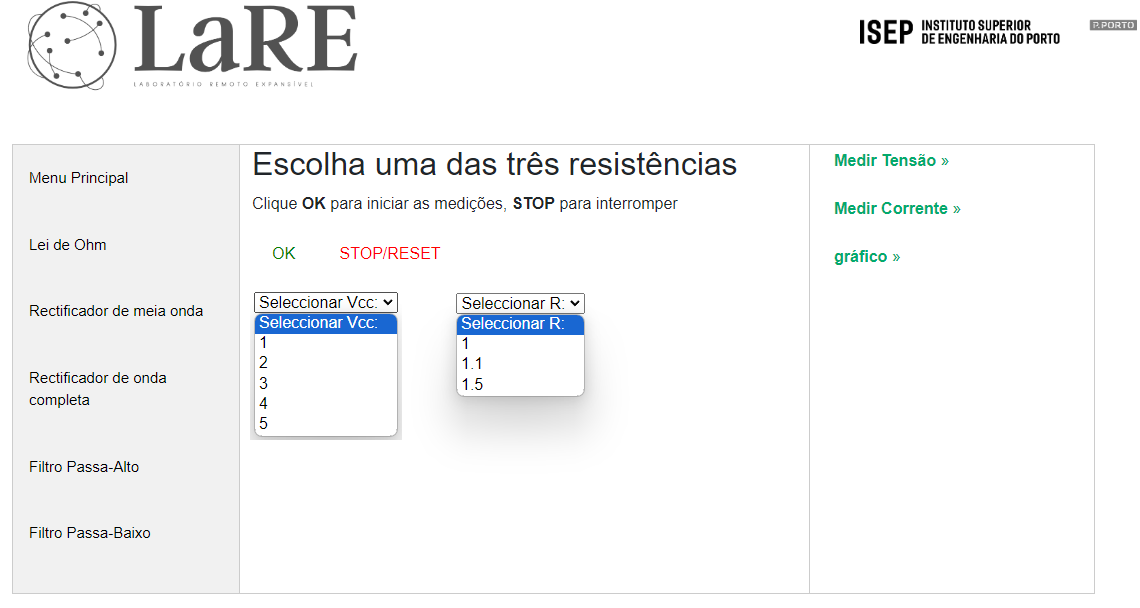
\includegraphics[width=6.3cm]{figures/ohm_escolha.png} }}%
		\qquad
		\subfloat[\centering Opção 2\label{fig:Opção_2}]{{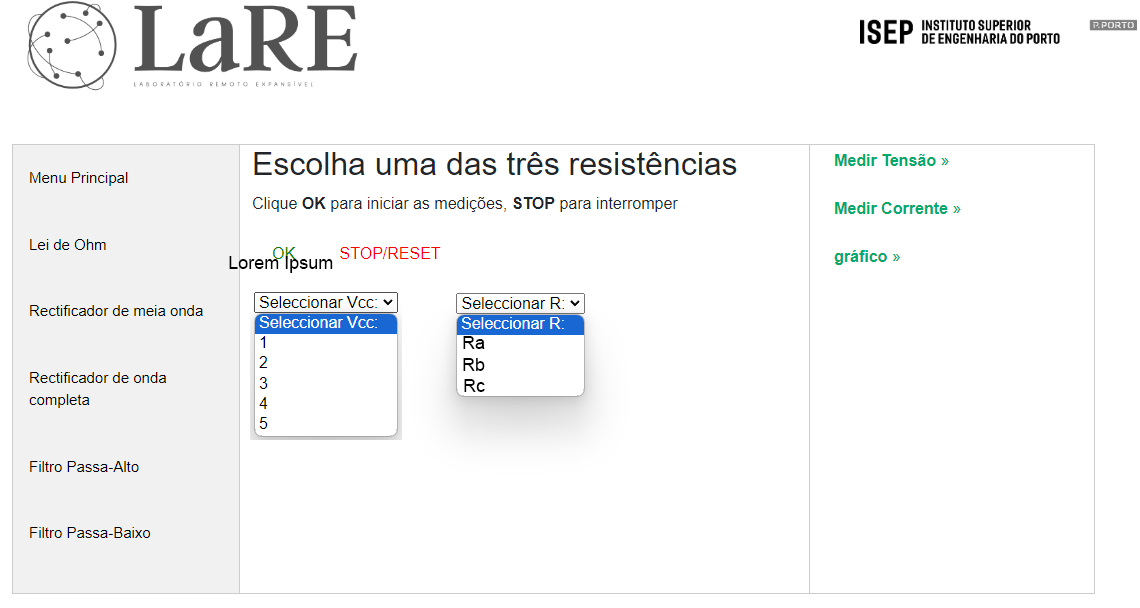
\includegraphics[width=6.3cm]{figures/ohm_escolha_abc.png} }}%
		\caption{Experiência Lei de \textit{Ohm}}%
		\label{fig:experienciaOHM}%
	\end{figure}
O tutor ou professor, pode optar por apresentar o conceito de duas formas distintas, em ambos os casos são efectuadas cinco medições, construido o respectivo gráfico e calculado o valor do declive da recta analiticamente. A diferença está na forma como se confrontam os resultados práticos. 

No caso em que a resistência é dada, o declive pode ser calculado e confrontado com as soluções, sendo que no caso em que é desconhecida, o declive da recta é calculado e a partir deste do resultado infere-se o valor da resistência. 

\textbf{Tal como o prof disse, refrerir que os valores, imagem, iformação e enviada para a página via xpto, blá, blá, através do ficheiro, flask, tal como referido no cap tal - referir também como é enviada a string}

\textbf{Falta o complemento com imagens do gráfico/resultado final e a imagem da placa já feita, opinião PROF}


\section{Rectificadores}
A implementação destas duas experiências foi feita de forma a que se possa estudar e avaliar o \textit{ripple} dos rectificadores, consoante as quatro combinações possíveis dos pares resistência/condensador. No caso da rectificação de meia onda, é ainda possível variar a frequência entre os \SI{50}{\hertz} e \SI{2000}{\hertz} mas no caso da rectificação de onda completa, a frequência é fixa ao valor da rede eléctrica - \SI{60}{\hertz}.

\textbf{Tal como o prof disse, refrerir que os valores, imagem, iformação e enviada para a página via xpto, blá, blá, através do ficheiro, flask, tal como referido no cap tal - referir também como é enviada a string}

No caso dos rectificadores, o Bloco 1 fica reduzido ao gerador de sinal, sendo que esta configuração permite estudar a variação da tensão de \textit{ripple} com a frequência ou ao transformador monofásico. \textbf{Nota: Complementar com a foto da placa da fonte} O Bloco 2, depende do tipo de rectificador que se pretende estudar - um díodo ou uma ponte rectificadora, item \ref{diodos}. O Bloco 3 é o único bloco comum às duas experiências. Embora no estudo da rectificação de meia onda se use, somente, os componentes descritos nos itens \ref{resistencias} e \ref{condensadores}, já na implementação dos filtros, usou-se mais um condensador e uma resistência, descritos no item \ref{rescond}. 

Dentro do rectângulo tracejado a laranja, encontram-se os componentes do filtro dos rectificadores, sendo que, para o estudo dos filtros, são usados, também, os componentes dentro do rectângulo tracejado magenta.


\subsubsection{Filtros}
\label{sec:filtros}
Representados na Figura \ref{fig:filtrosesqgeral} estão os filtros simplificados, leccionados em contexto de sala de aula no ensino secundário.

A possibilidade de variar a frequência do sinal de entrada permite que estas experiências sejam utilizadas para estudar a resposta em frequência dos filtros, analisar o Diagrama de \textit{Bode}, determinar a frequência de corte dada pela Equação \ref{eq:frequenciacorte} e ainda relacionar, por exemplo, o valor da tensão de entrada com a tensão de saída. 

\begin{equation} \label{eq:frequenciacorte}
	f_{c} = \frac{1}{2\pi RC}
\end{equation}

\begin{comment}
	\textbf{Acho que não é necessário referir a relação entre a tensão de entrada e a tensão de saída, já que isso é feito na parte de software. O que se pode fazer é referir que o \acrshort{lare} permite estudar a resposta em frequência dos filtros, analisar o Diagrama de \textit{Bode} e determinar a frequência de corte.}
A Figura \ref{fig:diagramabode} apresenta um exemplo do Diagrama de \textit{Bode} de um filtro passa-alto, obtido nos testes do LaRE.

\begin{figure}[hbtp]
	\centering
	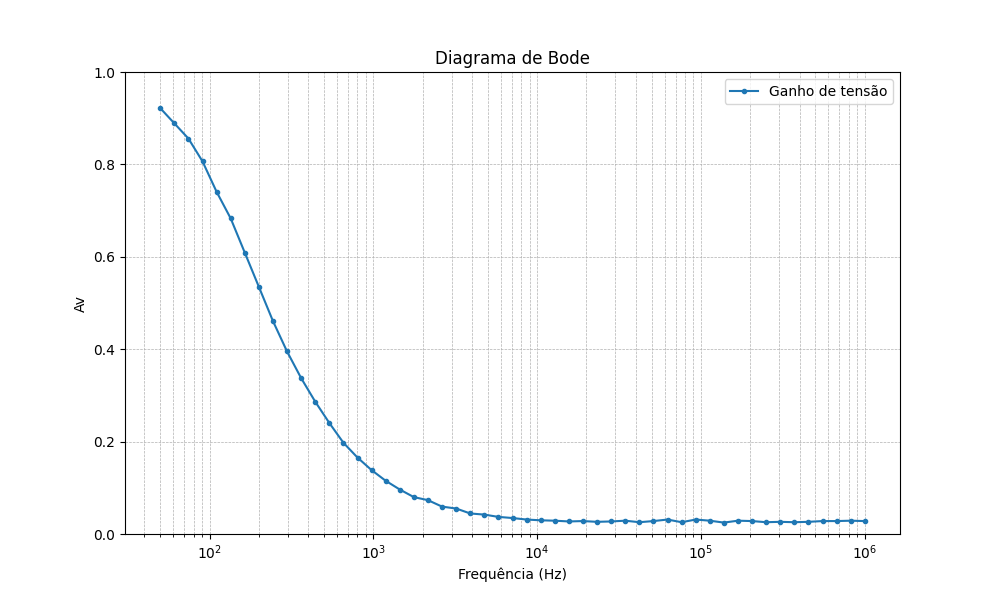
\includegraphics[width=0.6\textwidth]{figures/bode_lpf.png}
	\caption{Diagrama de \textit{Bode} - Filtro passa-alto}
	\label{fig:diagramabode}
\end{figure}
\end{comment}

As Figuras \ref{fig:Bode_pb} e \ref{fig:Bode_pa} apresentam os Diagramas de \textit{Bode} \textins{ideais}, que servem de referência para o estudo desta experiência. 

\begin{figure}[hbtp]
	\centering%
		\centering
		\subfloat[\centering Filtro passa-baixo\label{fig:Bode_pb}]{{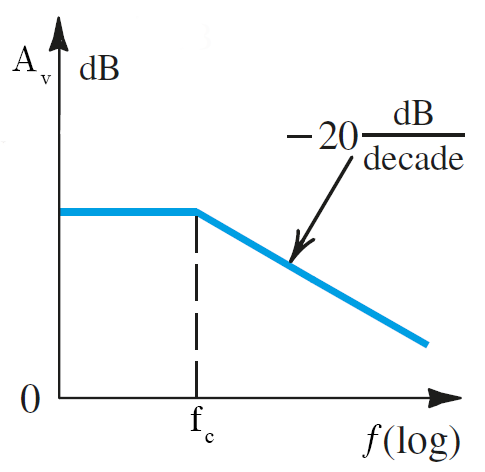
\includegraphics[width=6cm]{figures/Sedra_BodeFPB.png} }}%
		\qquad
		\subfloat[\centering Filtro passa-alto\label{fig:Bode_pa}]{{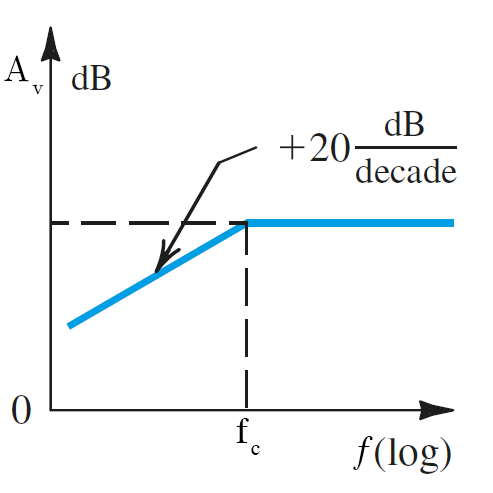
\includegraphics[width=6cm]{figures/Sedra_BodeFPA.png} }}%
		\caption{Diagramas de \textit{Bode} \textins{ideal} \cite{sedrasmith}}%
		\label{fig:Bodeesqgeral}%
\end{figure}

	Para além da análise em frequência, um outro aspeto complementar a considerar é a relação entre as ondas de entrada e saída, em função da frequência. Nos filtros, o intervalo de frequências permitido é igual ao já referido para os rectificadores: entre \SI{50}{\hertz} a \SI{2000}{\hertz}. 
	
	A frequência de corte de um filtro é definida como o ponto onde o ganho do filtro sofre uma atenuação de \SI{3}{\decibel} em relação ao seu valor máximo. 	Para um filtro passa-baixo (passa-alto) ideal, o ganho em baixas (altas) frequências é unitário. Quando o sinal atinge a frequência de corte, a relação entre a tensão de saída e a tensão de entrada reduz-se para:  
	
	\begin{equation} \label{eq:relacaoGanho}
		\frac{U_{out}}{U_{in}} = \frac{1}{\sqrt{2}} \approx 0.707
	\end{equation}
	
	\ldots ou na escala logarítmica:  
\begin{equation} \label{eq:relacaoGanhodB}
	\frac{U_{out}}{U_{in}} = 20 \log_{10} (0.707) \approx -\SI{3}{\decibel}	
\end{equation}
	
Assim, a frequência de corte de um filtro corresponde ao ponto em que a amplitude do sinal de saída é aproximadamente $70.7\%$ da amplitude do sinal de entrada, o que corresponde a -\SI{3}{\decibel}. 


\textbf{Tal como o prof disse, refrerir que os valores, imagem, iformação e enviada para a página via xpto, blá, blá, através do ficheiro, flask, tal como referido no cap tal - referir também como é enviada a string}

\textbf{DE UMA FORMA BREVE E RESEUMIDA, REFERIR QUANTO BITS E COMO SE FAZ A COMUNICAÇÃO COM O SER}

13 bits começar pelo esquema completo antes de dar os exemplos de funcionamento. a explicação penso que pode ficar dividida como está, mas já com o esquema e relés com os indices certos, a explicação mas os exemplos descritos em tabela só fazem sentido se for o esquema completo,


\section{Limitações}
\section{Melhoramentos}


